\documentclass{standalone}
\usepackage{tikz}

\begin{document}

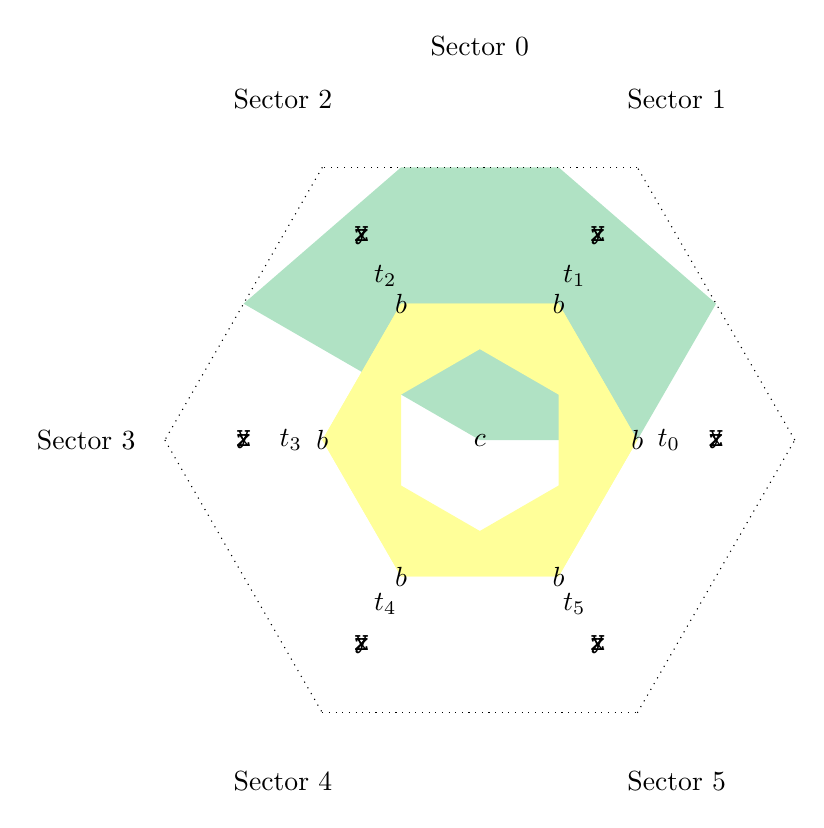
\begin{tikzpicture}[scale=2]
    % Define colors
    \definecolor{lightyellow}{RGB}{255, 255, 153}
    \definecolor{lightgreen}{RGB}{176, 226, 196}
    
    % Draw the main hexagon
    \fill[lightgreen] (0,0) -- (1,0) -- (1.5,0.866) -- (0.5,1.732) -- (-0.5,1.732) -- (-1.5,0.866) -- cycle;
    
    % Draw the sectors
    \foreach \i in {0,...,5} {
        \draw[dotted] ({\i*60}:2) -- ({(\i+1)*60}:2);
    }
    
    % Draw the triangles
    \foreach \i in {0,...,5} {
        \fill[lightyellow] ({\i*60}:1) -- ({(\i+1)*60}:1) -- ({(\i+2)*60}:1) -- cycle;
        \node at ({\i*60}:1.2) {$t_{\i}$};
        \node at ({\i*60}:1.5) {\texttt{x}};
        \node at ({(\i+1)*60}:1.5) {\texttt{y}};
        \node at ({(\i+2)*60}:1.5) {\texttt{z}};
    }
    
    % Label the sectors
    \node at (0,2.5) {Sector 0};
    \node at (60:2.5) {Sector 1};
    \node at (120:2.5) {Sector 2};
    \node at (180:2.5) {Sector 3};
    \node at (240:2.5) {Sector 4};
    \node at (300:2.5) {Sector 5};
    
    % Draw the center labels
    \node at (0,0) {$c$};
    \node at (60:1) {$b$};
    \node at (120:1) {$b$};
    \node at (180:1) {$b$};
    \node at (240:1) {$b$};
    \node at (300:1) {$b$};
    \node at (360:1) {$b$};
\end{tikzpicture}

\end{document}